\documentclass{article}
\usepackage[utf8]{inputenc}
\usepackage[T1]{fontenc}
\usepackage{graphicx}
\usepackage{hyperref}
\usepackage{geometry}
\geometry{margin=1in}

\title{NAXO}
\date{Encyclopaedia Britannica (1771)}

\begin{document}
\maketitle

\section*{Historical source}
\textbf{Entry ID:} \texttt{entry-naxo-1268} \\
\textbf{Volume ID:} 194474782 \\
\textbf{Character Count:} 375

\subsection*{Extracted Text}
NAXO, a small island in the Eastern Soss, near to the north coasts of Golden, Long Bay, 34. 2. Lat. 1. 28. N.

NAXIESS are the majority of the Malabra coast. We may with truth affirm that they are the oldest notably in the world, for the mean ancient written mention them, and onto the far which permits the Mayre ladies to have several islands, ever once being allowed four.



\section*{Source record}
\begin{itemize}
\item \textbf{Dataset:} \texttt{NationalLibraryOfScotland/encyclopaedia\_britannica\_illustrated}
\item \textbf{Dataset Revision:} \texttt{309f765b1ecc83e0a7f7762e44b4a927a7555443}
\item \textbf{Page ID:} \texttt{britannica:309f765b1ecc83e0a7f7762e44b4a927a7555443:train:1268} \\
  \textbf{Filename:} \texttt{page-1268-e5ec9e5b4086.jpg} \\
  \textbf{Row Index:} 1268 \\
  \textbf{SHA256:} \texttt{e5ec9e5b4086576d...}
\end{itemize}

\begin{figure}[h]
\centering
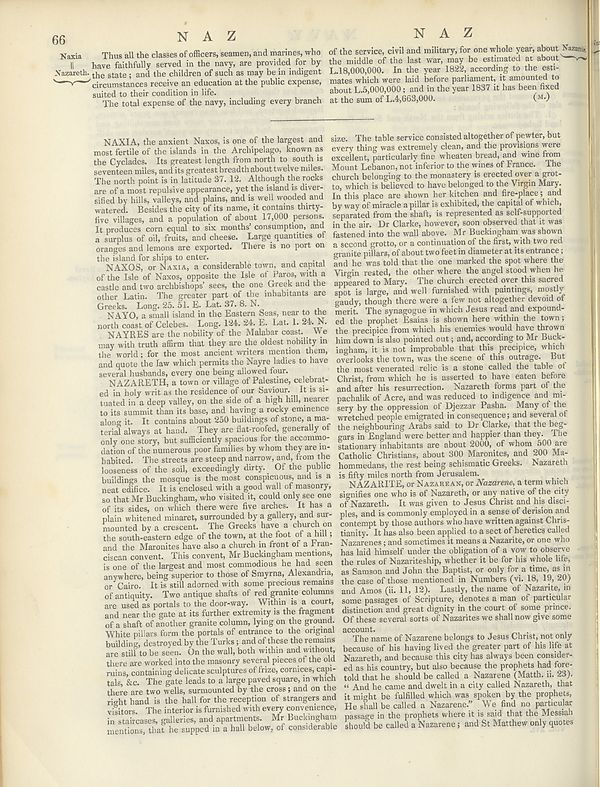
\includegraphics[width=0.85\textwidth]{../scans/page-1268-e5ec9e5b4086.jpg}
\caption*{Source scan: \texttt{page-1268-e5ec9e5b4086.jpg}}
\end{figure}

\end{document}
